\subsection{Третий этап. Тепловой шум и рассинхронизация}

На данном этапе производится учёт части искажений, возникающих при передаче сигнала через канал связи. Прежде всего, происходит наложение теплового шума (причины возникновения и математическое описание даны в разделе 3.b.i). Кроме того, вводятся временная и частотная рассинхронизация передатчика и приёмника (см. раздел 4.a). 

На рис. \ref{fg:schem3} выделены блоки, добавляемые на данном этапе. Рассмотрим подробно параметры, вводимые в модель.

\begin{figure}[h!]
\centering
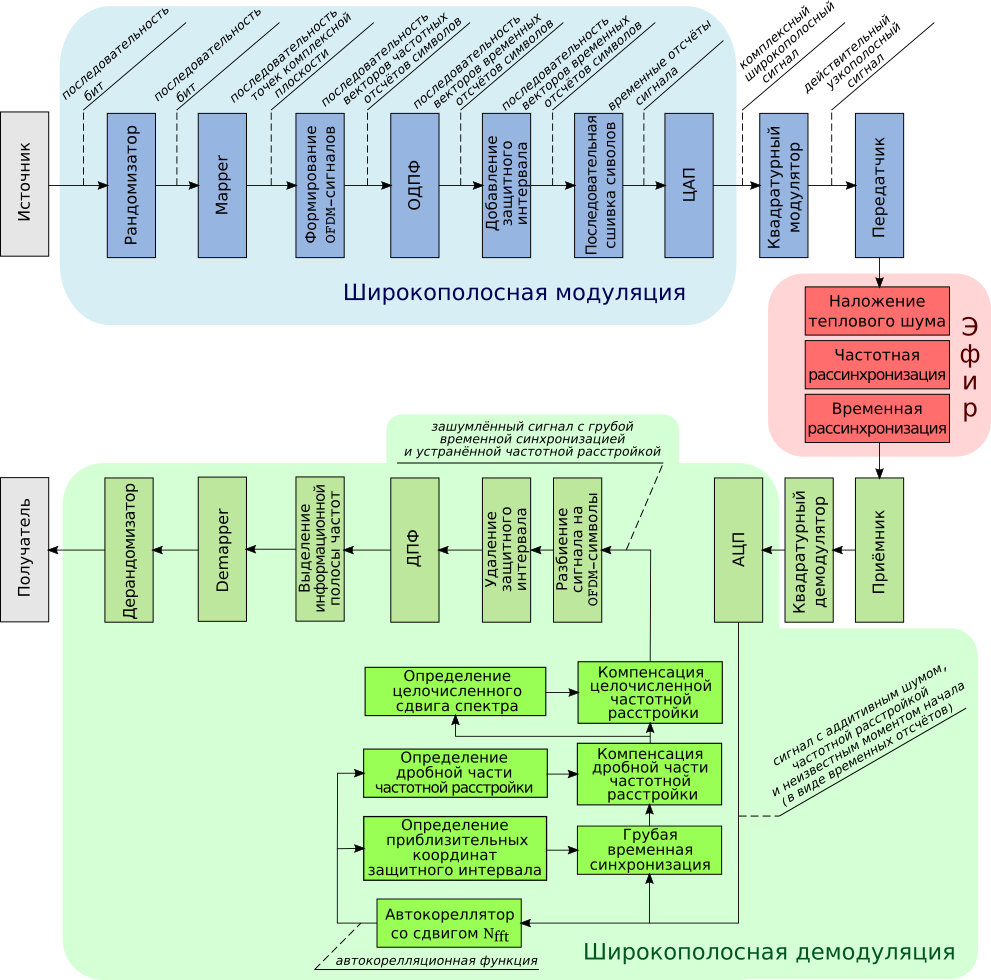
\includegraphics[width=1\textwidth]{OFDM-3.png}
\caption{Схема модели на третьем этапе} \label{fg:schem3}
\end{figure}

\subsubsection{Передающая сторона}
Структура передающей стороны на данном этапе не требует изменений.

\subsubsection{Канал}
В канале вводятся 3 вида искажений:
\begin{enumerate}
\item 
Тепловой шум. В радиоканале накладывается аддитивный гауссовский шум, мощность которого задаётся параметром \textit{отношение сигнал-шум (SNR)}. Поскольку в предполагается работа только с цифровым интерфейсом системы, на принимаемый сигнал необходимо накладывать вектор комплексного белого гауссовского шума с заданным \textit{SNR} (\textit{SNR} порядка $30\ dB$ считается высоким (а шум, соответственно, слабым), около $20\ dB$ -- низким).
\item		%Будет замечательно, если в теории по Фурье объяснить про единицы измерения времени и частоты в ДПФ
Частотная расстройка. Производится повышение частоты последовательности на задаваемую параметром \textit{freq\underline{ }shift} величину (в единицах отсчёта по частоте), что достигается умножением последовательности на комплексную экспоненту соответствующей частоты.
\item
Временная расстройка. Последовательность отсчётов сигнала сдвигается путём отбрасывания некоторого числа \textit{time\underline{ }shift} начальных отсчётов. Считать, что сдвиг кратен шагу дискретизации.
\end{enumerate}

\subsubsection{Принимающая сторона}
Непосредственно после получения цифрового сигнала и перед его обработкой проводят 3 этапа синхронизации:
\begin{enumerate}
\item
Грубая временная синхронизация (см. раздел …). Благодаря введению защитного интервала пропадает необходимость в точном нахождении начала символа для вычисления его ДПФ. Необходимо выбрать в качестве начала лишь некоторую точку в пределах защитного интервала. При этом, однако остаётся нескомпенсированный линейный набег фазы в спектре, который может быть устранён лишь при точной частотной синхронизации (см. этап 4).
\item
Дробная частотная синхронизация (см. раздел …). Сдвиг спектра на нецелое число отсчётов приводит к нарушению ортогональности несущих. Дробная часть этого смещения находится из автокорреляционной функции.
\item
Целочисленная частотная синхронизация (см. раздел …). Если спектр был смещён на величину, превышающую половину отсчёта ДПФ по частоте, возникает необходимость компенсировать и целочисленную часть смещения. Она легко находится из вида спектра.
\end{enumerate}
Для проведения первых двух этапов необходимо вычисление корреляции сигнала с его сдвинутой на \textit{n\underline{ }fft} копией. Ширина окна корреляции задаётся параметром \textit{Tw}.

\subsubsection{Вопросы и задания}
\begin{enumerate}
\item
Сгенерировать и наложить тепловой шум. Вычислить и проверить \textit{SNR} полученного сигнала без применения встроенных функций. Проверить эффективность восстановления данных и построить восстановленное созвездие. Что обеспечивает защиту данных от искажения тепловым шумом?
\item
Ввести сдвиг сигнала на величину меньше \textit{Tg} и на величину в 2-3 раза больше \textit{Tg}. Для каждого случая построить модуль ДПФ для одного символа. Не забыть вырезать защитный интервал (обратите внимание, теперь он вырезается не из начала, а из конца символа). Чем объяснить разницу в картинках?
\item
Построить автокорреляционную функцию. Изучить зависимость её вида от ширины окна \textit{Tw} в пределах от минимального до \textit{Tg}. Какие значения этого параметра дают лучший результат и почему?
\item
Реализовать алгоритм приблизительного нахождения середины защитного интервала для любого смещения. Учесть, что возможно возникновение статистических выбросов, а за счёт наличия шума высоты плато автокорреляции оказываются ниже 1. Убедиться, что получаемая точка лежит в пределах защитного интервала.
\item
Компенсировать сдвиг обрезанием начальных отсчётов. Построить модуль ДПФ одного символа. Построить восстанавливаемое из символа созвездие. Почему оно закручивается?
\item
Ввести частотную расстройку абсолютной величиной менее 0.5. Построить модуль ДПФ для одного символа в отсутствие частотной синхронизации и с ней. Объяснить, почему так искажается форма спектра.
\item
Произвести частотную синхронизацию. С каким знаком бралось значение для компенсации расстройки и почему? Проверить ДПФ после синхронизации.
\item
Ввести частотный сдвиг на произвольную частоту порядка нескольких десятков отсчётов. Реализовать целочисленную подстройку частоты. Проверить, что модуль спектра восстановлен и не смещён. 
\item *
Для отлаженной схемы третьего этапа проведите следующий эксперимент: вместо <<честно>> найденной приблизительно середины защитного интервала подставьте точный номер отсчёта, следующего за защитным интервалом (начало основной части символа). Таким образом моделируется ситуация, якобы грубая синхронизация дала точный результат. Постройте получаемое созвездие. Должно получиться правильно восстановленное созвездие, однако оно может получиться наклонённым. Объясните природу возникновения этого наклона.
\end{enumerate}
Обратите внимание, что после выполнения заданий 3-го этапа исходная битовая последовательность перестанет восстанавливаться, так как созвездие <<закручивается>>. Этот недочёт будет исправлен лишь на следующем этапе. Принципиальным результатом, демонстрирующим успешное выполнение данного этапа, является восстановленный несмещённый модуль спектра.